\documentclass[output=paper]{langsci/langscibook} 
\author{Chaya R. Nove\affiliation{Graduate Center at City University of New York}}
\title[Language contact in Hasidic Yiddish]
      {Outcomes of language contact in New York Hasidic Yiddish}

\abstract{Hasidic Yiddish (HY), brought to the U.S. by post-Holocaust immigrants, is currently the native language of five generations of bilingual speakers in New York. In this new contact setting, a unified variety is emerging, which has diverged from its Eastern European Yiddish parent dialect(s). The present study is a bilingual comparison whose aim is to examine, for a subset of HY and English vowels, how early HY-English bilinguals organize their phonetic system(s), and to explore the degree and direction of cross-linguistic influence. To that end, twenty-four early HY-English bilinguals, eight per generation (starting with Gen2, the children of immigrants), were recorded reading monosyllabic HY and English CVC words containing the vowels /i, ɪ, u, ʊ, a/ (approximately 100 tokens per speaker, 10 of each vowel). Pillai scores were calculated for each vowel category by generational group to measure the extent of overlap in the category by language. For /u/, Pillai scores were calculated separately for the lexical sets TOO and HOOP, reflecting the implicational hierarchy attested in North American English in these contexts \citep{Fridland2008, Hall-Lew2009, LabovEtAl2005, Wong2014}. The findings suggest apparent time change between Gen2 and Gen3/Gen4 in two areas: 1) spectral overlap of /ɪ/ and /ʊ/ in the two languages; and 2) relative advancement of English vs. HY /u/. Specifically, HY and English high lax vowels are qualitatively distinct for the oldest generation but show greater convergence in the younger generations. Additionally, while Gen2 HOOP and TOO both overlap cross-linguistically, English /u/-sets of Gen3 and Gen4 show more fronting. The results are interpreted with reference to models of second language acquisition, emphasizing how differences in language input might result in the acquisition of different systems. This study illustrates how an understanding of the dynamic nature of the language systems of individual learners can help explain structural change observed in the language of a speech community.}
\IfFileExists{../localcommands.tex}{
  % add all extra packages you need to load to this file

\usepackage{tabularx,multicol}
\usepackage{url}
\urlstyle{same}

\usepackage{listings}
\lstset{basicstyle=\ttfamily,tabsize=2,breaklines=true}

\usepackage{langsci-optional}
\usepackage{langsci-lgr}
\usepackage{langsci-gb4e}
% \usepackage{langsci-plots}
\usepackage{pgfplots}

\usepackage{siunitx}
\sisetup{group-digits=false}

\usepackage{amssymb}% http://ctan.org/pkg/amssymb
\usepackage{pifont}% http://ctan.org/pkg/pifont
\newcommand{\cmark}{\ding{51}}%
\newcommand{\xmark}{\ding{55}}%
% \usepackage[disable]{todonotes}
\usepackage{todonotes}

  \newcommand*{\orcid}{}
\newcommand{\hoederN}{n̡} 
  %% hyphenation points for line breaks
%% Normally, automatic hyphenation in LaTeX is very good
%% If a word is mis-hyphenated, add it to this file
%%
%% add information to TeX file before \begin{document} with:
%% %% hyphenation points for line breaks
%% Normally, automatic hyphenation in LaTeX is very good
%% If a word is mis-hyphenated, add it to this file
%%
%% add information to TeX file before \begin{document} with:
%% %% hyphenation points for line breaks
%% Normally, automatic hyphenation in LaTeX is very good
%% If a word is mis-hyphenated, add it to this file
%%
%% add information to TeX file before \begin{document} with:
%% \include{localhyphenation}
\hyphenation{
affri-ca-te
affri-ca-tes 
}
\hyphenation{
affri-ca-te
affri-ca-tes 
}
\hyphenation{
affri-ca-te
affri-ca-tes 
} 
  \togglepaper[1]%%chapternumber
}{}

\begin{document}
\maketitle 



\section{Introduction}
\label{sec:nove:1}

A frequent finding in research on migrant linguistic minority communities, is that shift to the dominant language is typically complete within three generations of arrival (see e.g., \citealt{Alba2004, AlbaEtAl2002, RumbautEtAl2006}).\footnote{I wish to thank Bill Haddican (Queens College) and Juliette Blevins (CUNY Graduate Center) for advisement; Arianna Chinchilla, April Polubiec, and Nutti Gross for assistance with data processing; Danielle Ronkos for feedback on an early version of this chapter; and the editors of this volume and two anonymous reviewers for their valuable comments and suggestions. I am grateful to the following organizations for research funds: Endangered Language Initiative (ELI GC CUNY); Doctoral Studies Research Grant (GC CUNY); and Center for Jewish Studies (GC CUNY).} This trend has been observed following both past and recent waves of immigration and was formalized as the \textsc{three-generation} \textsc{rule} (\citealt{Fishman1972, Haugen1953}). Diaspora immigrant groups that have defied these odds and retained their native vernacular beyond three generations are valuable testing sites for theories of language variation and change. 

The present research focuses on one such language. Hasidic Yiddish (HY)\footnote{The term Hasidic Yiddish as used here excludes the Yiddish spoken in Lubavitch (Chabad) communities, which derives from Northeastern Yiddish varieties and differs significantly from the Hasidic Yiddish originating from the Central Yiddish dialects. While I resort to this term for the sake of simplicity, I acknowledge that excluding Lubavitch Yiddish renders it somewhat problematic.}  has been transmitted by post-Holocaust refugees from Eastern Europe and is currently the native language of five generations of Hasidic [ultra-Orthodox] Jews in New York State.\footnote{While New York has the highest concentration of HY speakers in North America, there are also HY-speaking communities in New Jersey, California, Montreal and Toronto. Across the world, sizable HY-speaking groups can be found in Israel, England (London) and Belgium (Antwerp) \citep{Assouline2018}.} This study examines the degree and direction of crosslinguistic influence resulting from stable bilingualism by comparing the phonetic similarity of vowels in speakers’ first and second languages (HY and American English, respectively). The analysis is based on tokens of HY and English /i, ɪ, u, ʊ, a/, produced by twenty-four speakers representing three generational groups. Vowel formant frequencies are compared across language and generation to identify change over time. The results show crosslinguistic differences in the acoustic correlates of /ɪ/, /ʊ/, and /u/ for second and third generation speakers. The findings are interpreted with reference to theories developed in the field of second language acquisition studies (henceforth, SLA), highlighting the sociohistorical circumstances that resulted in dissimilar language input across these groups. 

As a quantitative sociolinguistic analysis of a minority language community, this study hews closely to the research goals that shaped the field of modern sociolinguistics.\footnote{Modern sociolinguistics is rooted in issues related to language contact (see \citealt{Weinreich1970}), however, the research paradigm in the field shifted to monolingual communities early on (e.g., \citealt{labov_social_2006}), in large part due to the challenges inherent in studying multilingual communities (see \citealt{Sankoff2002}). More recently there has been a call by sociolinguists for more quantitative research of minority languages and multilingual contexts (see \citealt{GuyAdli2019, NagyMeyerhoff2008, Stanford2016}).} The application of SLA models situates this paper within a comparatively more recent tradition in the field that promotes an inter-disciplinary approach between variationist sociolinguistics and SLA (see e.g., \citealt{AdamsonRegan1991, Bayley2000, FasoldPreston2007, PrestonBayley1996, Regan2004, Tarone2007, YaoChang2016}). 

The remainder of this chapter is organized as follows: In \sectref{sec:nove:2}, relevant sociohistorical and sociocultural details will be provided to acquaint the reader with the circumstances of New York HY. \sectref{sec:nove:3} introduces the Speech Learning Model (SLM) of second language acquisition developed by \citet{Flege1995, Flege1996}. The data, methods and results of the study are described in \sectref{sec:nove:4}. \sectref{sec:nove:5} discusses the findings in the context of SLA and offers some concluding remarks.  

\section{Background}
\label{sec:nove:2}


\subsection{Hasidic Yiddish in New York}
\label{sec:nove:2.1}

HY is exceptional both as a U.S. minority language that has resisted the trend towards language shift,\footnote{Languages spoken by auto-segregated religious groups often withstand the three-generation rule. Pennsylvania German (also known as Pennsylvania Dutch) is another example of a Germanic minority language in the United states whose retention has been attributed to socio-religious factors, and which has been explicitly compared to Hasidic Yiddish \citep{Louden2016}.} and as a Yiddish variety that has thrived while its sister dialects globally declined to the point of virtual obsolescence in the decades following WWII. It is currently the native language of 135,000--273,000 Hasidic Jews\footnote{This range is based on the 2011--2015 American Community Survey of the U.S. Census Bureau \citep{MansonEtAl2017} and approximations offered by \citet{BialeEtAl2018} of the number of Hasidim in Greater New York, who are presumed to be Yiddish speakers.} in New York State and its environs, where the speaker population has been increasing steadily due a unique combination of demographics and ideology: A high birth rate within the Hasidic community leads to natural population growth, while HY use is promoted as a means of ensuring cultural separatism and religious continuity (\citealt{Fishman1965Yiddish, Shandler2006, Fader2009, Glinert1999}). \figref{fig:nove:1} shows the locations of the largest Hasidic communities in New York. 

\begin{figure}
\centering
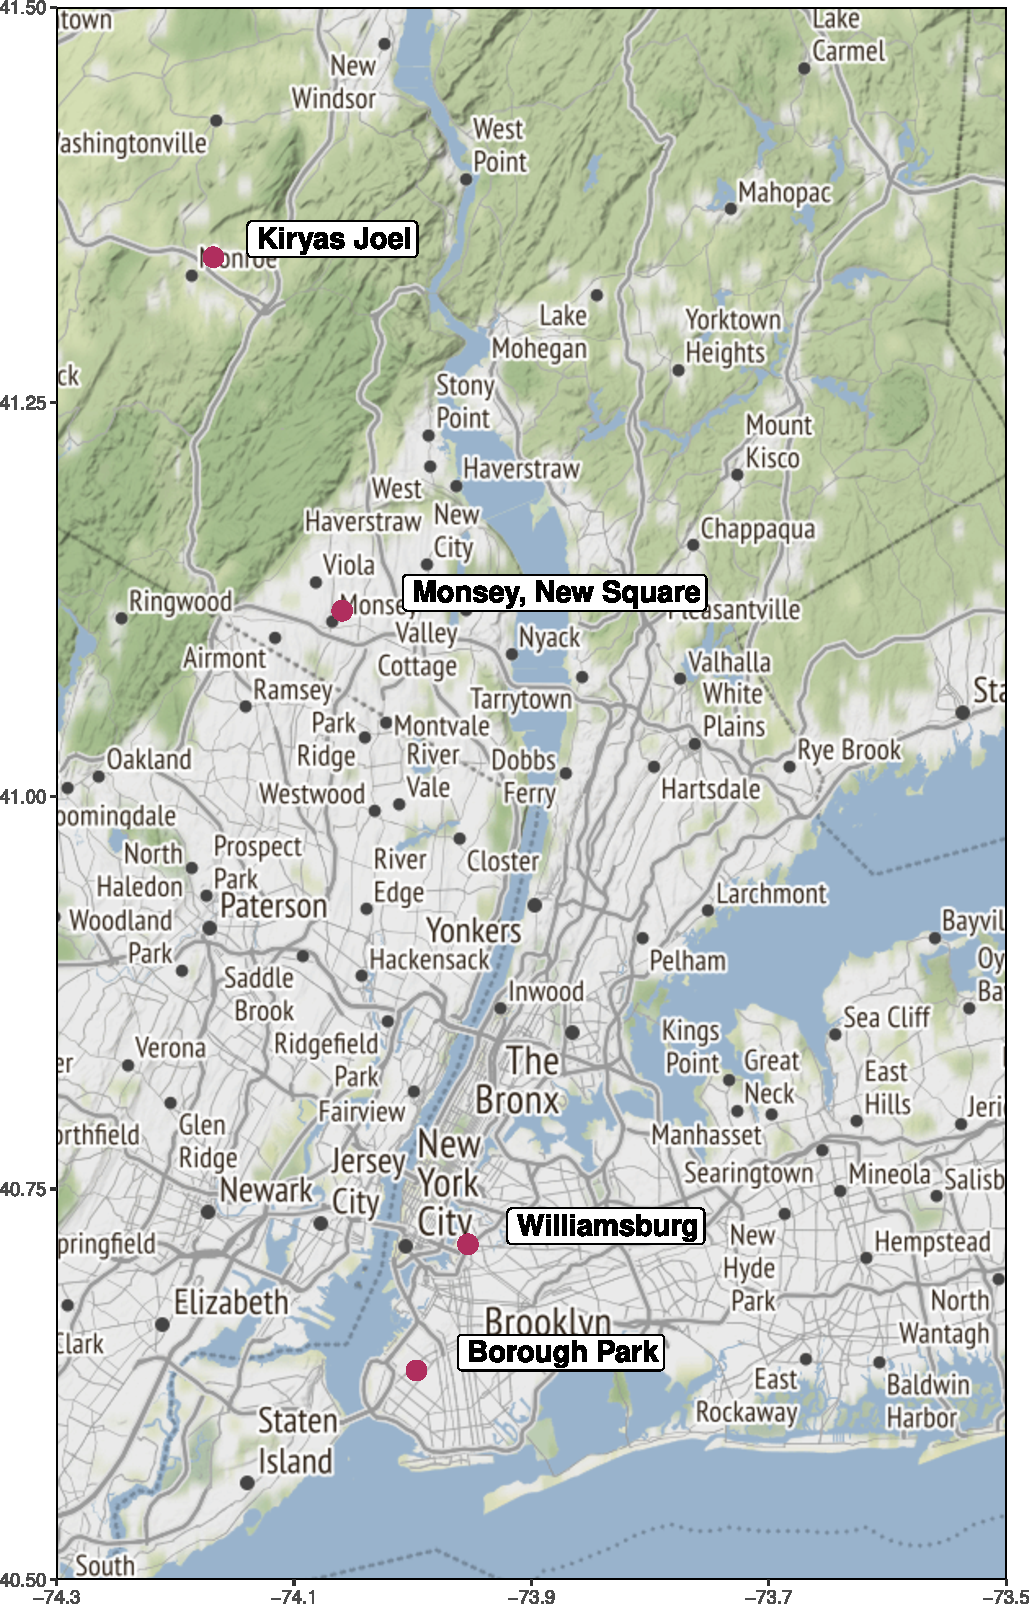
\includegraphics[width=0.8\textwidth]{figures/nove-fig1-color.pdf}
\caption{New York Hasidic Communities: Map showing  locations of the four largest Hasidic communities in New York State (map created using the ggmap package, \citealt{KahleWickham2013}, in R software, \citealt{RCore2017}}\label{fig:nove:1}
\end{figure}


HY derives from the dialects spoken in the pre-war Eastern European region referred to by Yiddish-speaking residents as the Unterland,\footnote{The terms \textit{Oyberland} and \textit{Unterland} overlap semantically with Hungarian \textit{Felföld} (Highland) and \textit{Alföld} (Lowland). However, while the latter refer to a north/south territorial division, the former designate a west/east division that was culturally relevant to Yiddish-speaking residents of formerly Hungarian territories \citep{Weinreich1964}.} which roughly corresponds to the border area of modern-day Slovakia, Hungary, Ukraine, and northwestern Romania and central Romania, as illustrated by the area highlighted in \figref{fig:nove:2} (\citealt{Weinreich1964}; \citealt{Krogh2012}). Yiddish dialectologists include the historical Unterland in the Central Yiddish (CY) dialect region.\footnote{Eastern Yiddish is discussed in terms of three main dialect groups: Northeastern Yiddish originated in what is currently Lithuania, Belarus, Latvia, areas of northeastern Poland, northern and eastern Ukraine, and western Russia; Southeastern Yiddish was spoken in Moldova and parts of Ukraine; and Central Yiddish was found in modern-day Poland, eastern Slovakia, eastern Hungary and Romania, including the historical Unterland region.} However, plurilingualism and dialect mixing was endemic to this particular geographical region, whose political borders shifted frequently. Moreover, some of the HY-speaking groups in New York trace their ancestry to locations beyond the Unterland (e.g., the Bobov Hasidic group, from Bobowa, Poland). Despite these somewhat eclectic dialectal origins, a unified variety of HY has emerged, which has only recently gained the attention of linguistic scholars (\citealt{Nove2018a}; \citealt{SadockMasor2018}). 

%%[Warning: Draw object ignored]
%{}-  
%%please move the includegraphics inside the {figure} environment
%%
 
\begin{figure}
%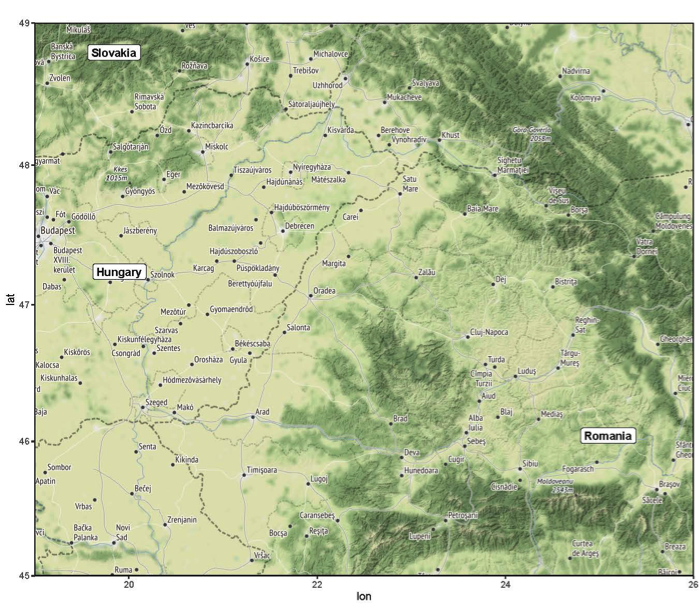
\includegraphics[width=\textwidth]{figures/a03Nove-img002.jpg}
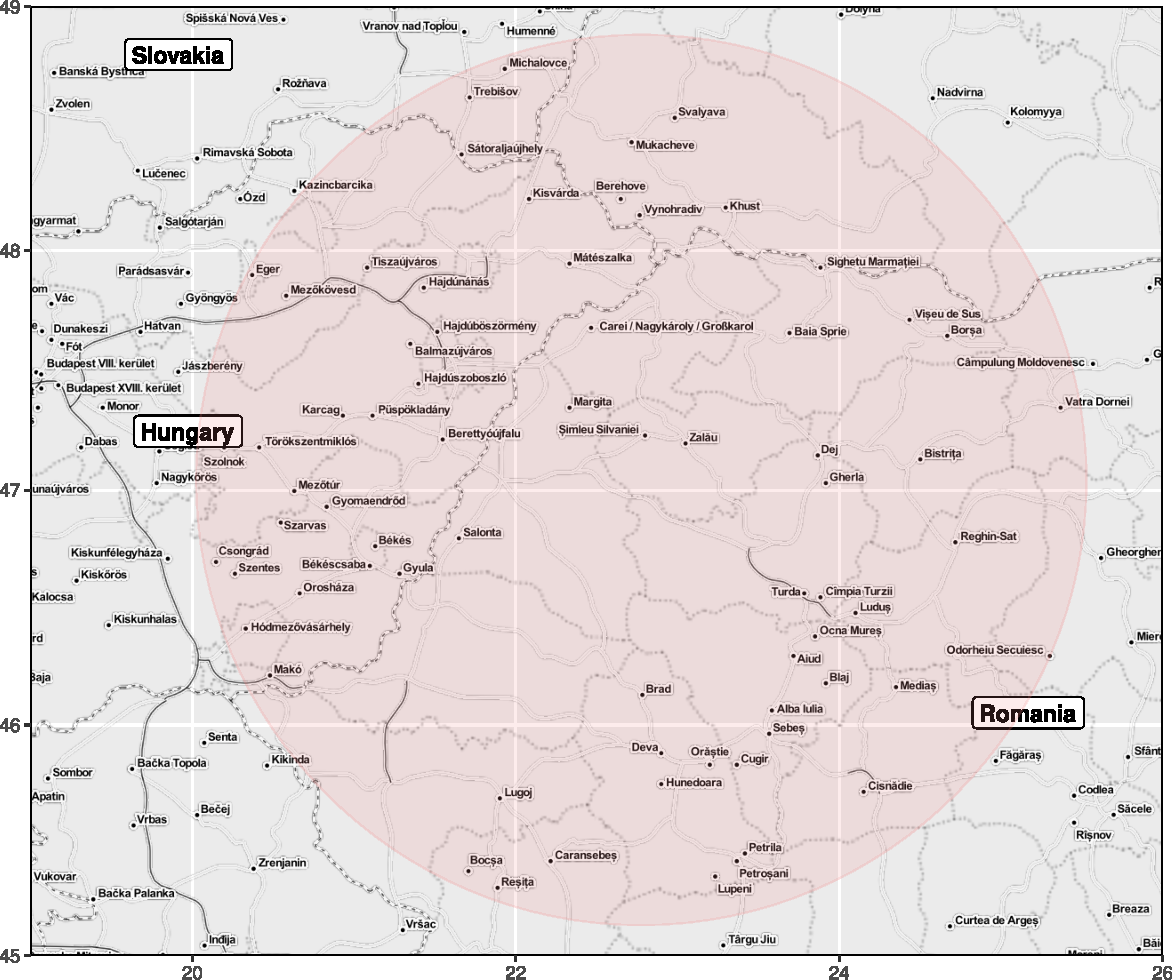
\includegraphics[width=\textwidth]{figures/nove-fig2-gray.pdf}
\caption{ Historical Unterland Region: Map showing the approximate pre-WWII Unterland region in Eastern Europe (map created using the ggmap package,\citealt{KahleWickham2013}, in R software, \citealt{RCore2017})}\label{fig:nove:2}
\end{figure}

 
\subsection{Sociocultural context}
\label{sec:nove:2.2}


The greater Hasidic community in the New York area is comprised of more than a dozen groups of various sizes, each united around a spiritual leader (\textit{rebbe}) and named after the pre-war Eastern European town or village from which the group originated.\footnote{Unless otherwise cited, sociocultural information is based on my fieldwork.} The most prominent of these is Satmar, whose name derives from present-day Satu Mare, Romania.\footnote{Detailed sociological studies of New York Hasidim are offered in \citet{Heilman1992, Heilman2017}, \citet{Kranzler1995}, \citet{Poll1962}, and \citet{Rubin1972, Rubin1997}. \citet{Fader2009} provides an in-depth ethnography of one New York Hasidic group. \citet{Wodzinski2018} compares the population sizes of contemporary Hasidic groups.} 

HY speakers are typically bilingual (with English),\footnote{Some liturgical Hebrew and Aramaic is also typically acquired via the oral translation of Hebrew and Aramaic texts to Yiddish.} but HY is acquired first and remains the dominant in-group language in many domains, including the home, the school and frequently also the workplace. Maintenance of the ancestral language is but one feature of the modern-day Hasidic ethos, which emphasizes traditionalism and cultural separatism. The Hasidic ideology is also manifested, inter alia, in gender segregation policies that govern virtually all aspects of social life and a distinctive dress code for men approximating that of 18\textsuperscript{th} century Jewish men in Eastern Europe.
 
 
Hasidic children are educated in private (gender-segregated) institutions overseen by the respective leaders of each Hasidic group. In the boys’ schools, the curriculum centers around religious studies with HY as the language of instruction, however, boys are rarely required to write in HY and prescriptive grammar is not taught \citep{Bleaman2018}. Approximately 60--90 minutes is devoted to secular subjects daily. In the girls’ schools, half of the (7-hour) school day is allocated to religious studies, taught in HY, and the other half to secular studies, with English as the instructional medium. HY literacy is taught, but minimal emphasis is placed on prescriptive norms. English grammar, on the other hand, is taught extensively from first grade through high school. Consequently, Hasidic males and females exhibit different patterns of HY-English bilingualism. 
 

\subsection{Length contrast in Yiddish vowels}
\label{sec:nove:2.3}

To date, very few acoustic analyses of HY have been reported. The following description is based on impressionistic and acoustic analyses of the data I have collected thus far. HY has twelve vowels in stressed syllables—eight monophthongs /a, aː, ɛ, i, ɪ, u, ʊ, ʌ/ and four diphthongs /aɪ, eɪ, ɔɪ, oʊ/. In unstressed position, these vowels neutralize to schwa. The inventory of HY monophthongs is shown alongside American English ones in \figref{fig:nove:3}. Note that HY high vowel pairs represented by the symbols /i, ɪ/ and /u, ʊ/ were likely /iː, i/ and /uː, u/ for Gen1/Unterland Yiddish speakers (see \citealt{Nove2020}; \citealt{Weinreich1964}); and that /ʌ/ corresponds to /ɔ/ in other Yiddish dialects.\footnote{An acoustic analysis of apparent time change from /ɔ/ to /ʌ/ is in progress.} 

%%THIS IS A FIGURE
\begin{figure}
%\begin{subfigure}[b]{0.4\textwidth}
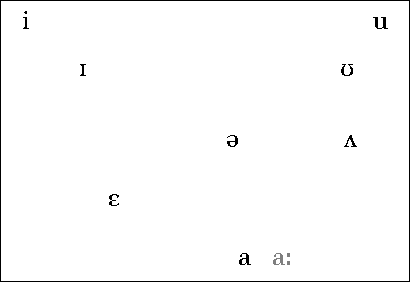
\includegraphics[width=0.5\textwidth]{figures/nove-fig3-1.pdf}
%\end{subfigure}
%\begin{subfigure}[b]{0.4\textwidth}
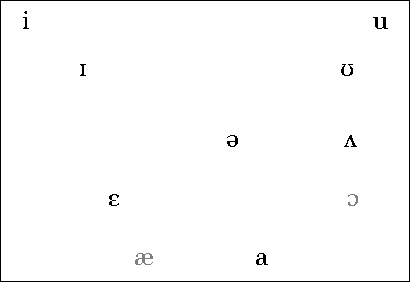
\includegraphics[width=0.5\textwidth]{figures/nove-fig3-2.pdf}
%\end{subfigure}
\caption{The inventory of HY (top) and American English (bottom) monophthong vowels. Vowels not common to both languages are shown in gray.} 
\label{fig:nove:3}
\end{figure}

A notable feature in HY, inherited from CY, is the contrast between long and short peripheral vowels /i/, e.g., [zin] ‘sons’ and [zɪn] ‘sun’; /u/, e.g., [ʃtruf] ‘punish’ and [ʃlʊf] ‘sleep’; and /a/, e.g., [haːnt] ‘today’ and [hant] ‘hand’.\footnote{In Standard Yiddish, the orthographic representations of these sample words are \textit{zin}, \textit{zun}, \textit{shtrof}, \textit{shlof}, \textit{haynt} and \textit{hant}, respectively.} In the literature on CY, this contrast is described in terms of length.\footnote{Central Yiddish is unique among Yiddish dialects in having maintained the Indo-European length feature in its vowel system. For in-depth analyses of the historical development of these vowels, I recommend \citep{Jacobs1990, Herzog1964}; and \citep{Beider2015}.} However, phonetic research has revealed a fair amount of complexity in the physical manifestation of vocalic length distinctions among the world’s languages,\footnote{For example, the spectral patterns of the long-short correlates of particular vowels in some languages show that longer sounds are produced with more muscular tension than shorter sounds (see e.g., \citealt{AbramsonRen1990}). Furthermore, perception experiments reveal that listeners may be more attuned to these qualitative differences than they are to differences in duration in some languages, for at least some vowels (see e.g., \citealt{AbramsonRen1990, Lehiste1970, PetersonLehiste1960}).} and the phonetics of CY vowels, absent acoustic analyses, is not known. A pilot study analyzing the vowels of three Unterland Yiddish speakers points to duration as the primary distinguishing feature between long-short peripheral vowels \citep{Nove2020}. Relatedly, in a study focusing on contemporary HY speakers, \citet{Nove2018b} describes the emergence of a tense-lax contrast for the high vowel pairs /i, ɪ/ and /u, ʊ/, but not in the long-short /aː, a/, which appear to differ primarily by relative duration. That is, while long and short /a/ exist in the same phonetic space, the short correlates of the high vowels are lower and more centralized than their long counterparts. Moreover, there is evidence of change over time, specifically a gradual lowering and centering of HY /ɪ/ and /ʊ/ between second and third generation speakers. The different trajectories of change in HY high vs. low vowels, with patterns of contrast in the high vowels becoming more similar to their English counterparts, while the /a/ pair, which lacks an equivalent in Northeastern American English, behaves differently, invites a contact-induced account of sound change.


\section{Modeling bilingualism}
\label{sec:nove:3}

 
\subsection{Language contact in sociolinguistic and SLA studies} 
\label{sec:nove:3.1}


Language contact phenomena, while notoriously difficult to isolate, are a potentially significant factor underlying language variation and change and are thus of great interest to sociolinguists conducting research in multilingual communities. It is also a point at which sociolinguistics interfaces with SLA studies; however, the approaches differ significantly between these two fields. While the bilingual individual has remained the central focus in SLA studies, research in the field of sociolinguistics focuses on patterns of language use in the speech community as a whole (\citealt{YaoChang2016, Sankoff2002}). The latter approach has facilitated a growing understanding of the linguistic and social factors that underlie language variability and change; however, it has provided less insight into cognitive factors that give rise to it. Scholars in both fields will undoubtedly agree that “[FEFF?]macro change (in the language of a speech community) starts with micro change (in the idiolect of a member of that community)” (\citealt{YaoChang2016}: 433). Using this unifying statement as a guiding principle, Yao and Chang demonstrate how an integrated approach combining SLA models of the speaker’s internal state with aggregated data obtained from a language community leads to a more detailed account of the status of a vowel merger in Shanghainese. The authors suggest that sociolinguistics can function as a testing site for models of SLA, for the mutual benefit of both fields.

Informed by the study cited above, the analysis provided in this paper layers an SLA approach onto data obtained via sociolinguistic methods for the purpose of identifying which of the observed patterns are attributable to language contact. Specifically, predictions about L1--L2 sound interaction in a bilingual speaker’s mind are used to interpret group data comparing the phonetic properties of HY and English vowels, for an account of contact-induced change in apparent time.\footnote{Based on an assumption that childhood speech patterns remain relatively stable across the lifespan, apparent time studies attempt to capture language change by examining an age-stratified cross section of a population at a particular point in time rather than longitudinally.} 


 
\subsection{The Speech Learning Model}
\label{sec:nove:3.2}


The Speech Learning Model (SLM), developed by \citet{Flege1995, Flege1996}, is based on the premise that mechanisms of language learning remain operative across the lifespan. Indeed, \citet{Flege2007} argues that the differential degrees of L2 acquisition long observed among second language learners are not attributable solely to maturational constraints (i.e., to a critical period), as many scholars have posited. Flege explains how age of L2 acquisition in studies of bilingualism are likely to be confounded by a number of other variables, chief among them the amount and quality of language input. 

While the phenomenon known as \textsc{interference} (the impact of L1 on the acquisition of L2 sounds) is well-known, the SLM is distinctive among other SLA models in explaining influence in the opposite direction. \citet{Flege1995, Flege1996} proposes that L1-L2 sound systems coexist in a shared phonological space in the bilingual mind and exert an ongoing bidirectional influence on each other. The interaction is based on a system of \textsc{equivalence} \textsc{classification}: L2 sounds that are perceived by learners as ‘new,’ i.e., acoustically distinct from sounds in the L1 inventory, will form new categories; while sounds that are perceived as ‘similar’ will be mapped onto acoustically similar L1 sounds, resulting in non-native production of those segments. (‘Identical’ sounds will similarly map onto L1 categories but will not result in any discernible production differences due to their inherent acoustic similarity.) He further explains that both language systems remain malleable throughout the lifespan. As the L1 system develops, it has an increasing (obstructive) influence on L2 learning, leading to outcomes often attributed to maturational constraints. Similarly, greater familiarity with, and use of, the L2, can lead to slight alterations in the phonetic quality of overlapping (similar) sounds, sometimes shifting them in the directions of the L2. Indeed, such change in the L1 as a consequence of experience with an L2, referred to as \textsc{phonetic} \textsc{drift,} is well attested in L2 dominant environments (see e.g., \citealt{Flege1987} on English learners of French in Paris and French learners of English in Chicago; and \citealt{SancierFowler1997} on Portugese learners of English both in Brazil and in the U.S.) as well as in environments where the L1 is predominantly spoken (see e.g., \citet{HerdEtAl2015} on English learners of Spanish in the U.S.). Moreover, in a study of English speakers learning Korean in South Korea, \citet{Chang2012, Chang2013} discovered that phonetic drift (at the subsegmental, segmental and global levels) was evident within the first two weeks of language learning, and indeed, that its effect was even more pronounced during early exposure. The author suggests drift is actually reduced as the learner’s familiarity with the L2 increases and points out that these results support a view of the L1-L2 systems as constantly evolving.  


\section{Data, methods and results}
\label{sec:nove:4}


 
\subsection{Data}
\label{sec:nove:4.1}


Data for this study were collected between June 2017 and February 2018. The sample consists of twenty-four native HY speakers, eight per generation (2, 3 and 4), where 2\textsuperscript{nd} generation (Gen2, etc., henceforth) refers to the children of post-Holocaust immigrants to the U.S. The age range for Gen2 is 60 – 70 (\textit{M} = 66.73, median = 68.5, \textit{SD} = 3.27) and five of them are female. Gen3 speakers range in age from 33 to 48 (\textit{M} = 38.88, median = 37.5, \textit{SD} = 5.39) and are balanced for sex. The Gen4 group is balanced for sex with an age range of 13 – 24 (\textit{M} = 17.51, median = 17, \textit{SD} = 4.17).  \tabref{tab:nove:1}, arranged by generation, lists the speakers’ ages and sex. 


\begin{table}
	\begin{tabularx}{\textwidth}{XXXXXXXXX}
	\lsptoprule
	\multicolumn{3}{X}{{Gen2}} & \multicolumn{3}{X}{{Gen3}} & \multicolumn{3}{X}{{Gen4}}\\
	{Speaker} & {Age} & Sex & {Speaker} & {Age} & Sex & {Speaker} & {Age} & Sex\\
	\hline
	 2A & 70 & F & 3A & 48 & F & 4A & 24 & F\\
	 2B & 69 & F & 3B & 39 & F & 4B & 20 & F\\
 	2C & 69 & F & 3C & 35 & F & 4C & 14 & F\\
 	2D & 68 & F & 3D & 33 & F & 4D & 13 & F\\
 	2E & 65 & F & 3E & 47 & M & 4E & 21 & M\\
 	2F & 69 & M & 3F & 38 & M & 4F & 21 & M\\
 	2G & 64 & M & 3G & 37 & M & 4G & 14 & M\\
 	2H & 60 & M & 3H & 34 & M & 4H & 13 & M\\
	\lspbottomrule
	\end{tabularx}
	\caption{List of speakers (with assigned codes) by generation, age and sex}\label{tab:nove:1}
\end{table}

Speakers were interviewed in a quiet room at a venue of their choice. The interview commenced with 30-40 minutes of open-ended conversation (not analyzed here). Next, participants were asked to repeat an HY carrier sentence, inserting a different Yiddish word with each repetition.\footnote{The carrier sentence was \textit{yetst} \textit{zog} \textit{X} \textit{shoyn} ‘now say X already.’} The stimuli (target words) were presented orthographically via digital flash cards (on a tablet), in a pseudo-randomized order. A cue card with the carrier sentence was visible to the speaker as the stimuli were presented. Finally, the above procedure was repeated for a list of English words. 

Yiddish and English stimuli included 8-10 monosyllabic content words for each of the five vowels relevant to this study (/i, ɪ, u, ʊ, a/).\footnote{Ten words for each vowel were initially included but some were not successfully elicited due to their unfamiliarity to speakers. A complete list of stimuli, along with a brief description of selection considerations, is included in \sectref{sec:nove:appendix}.}  

Data were recorded using a Zoom H4N digital audio recording device, with either a flat response, omnidirectional condenser lavalier microphone from Audio-Technica (AT899); or using the recorder’s built-in microphone.\footnote{The intention was to use the external microphone for all the interviews, but a flaw in the recorder’s software caused the device to occasionally switch to the built-in microphone mode. This problem went unnoticed for a while. The problem was eventually resolved by upgrading the software. A total of 9 out of 24 interviews analyzed here were recorded with the built-in microphone.}  The recordings were made in WAV format, with a sample frequency 44.1/kHz and a bit rate of 16.


 
 \subsection{Methods}
\label{sec:nove:4.2}


Audio files were imported to \textit{Praat} (\citealt{BoersmaWeenink2018}), where Textgrids containing transcriptions were generated. The sound segments in Yiddish words were aligned manually, while the English word files were aligned using Montreal Forced Aligner \citep{McAuliffeEtAl2017}. Sample segmented Yiddish and English word files (\textit{briv} ‘letter’ and \textit{beef}) are shown in \figref{fig:nove:4} and figref{fig:nove:5}. Misread words, words read in isolation (not in a carrier sentence) and words containing disfluencies were excluded from the analyses.


\begin{figure}
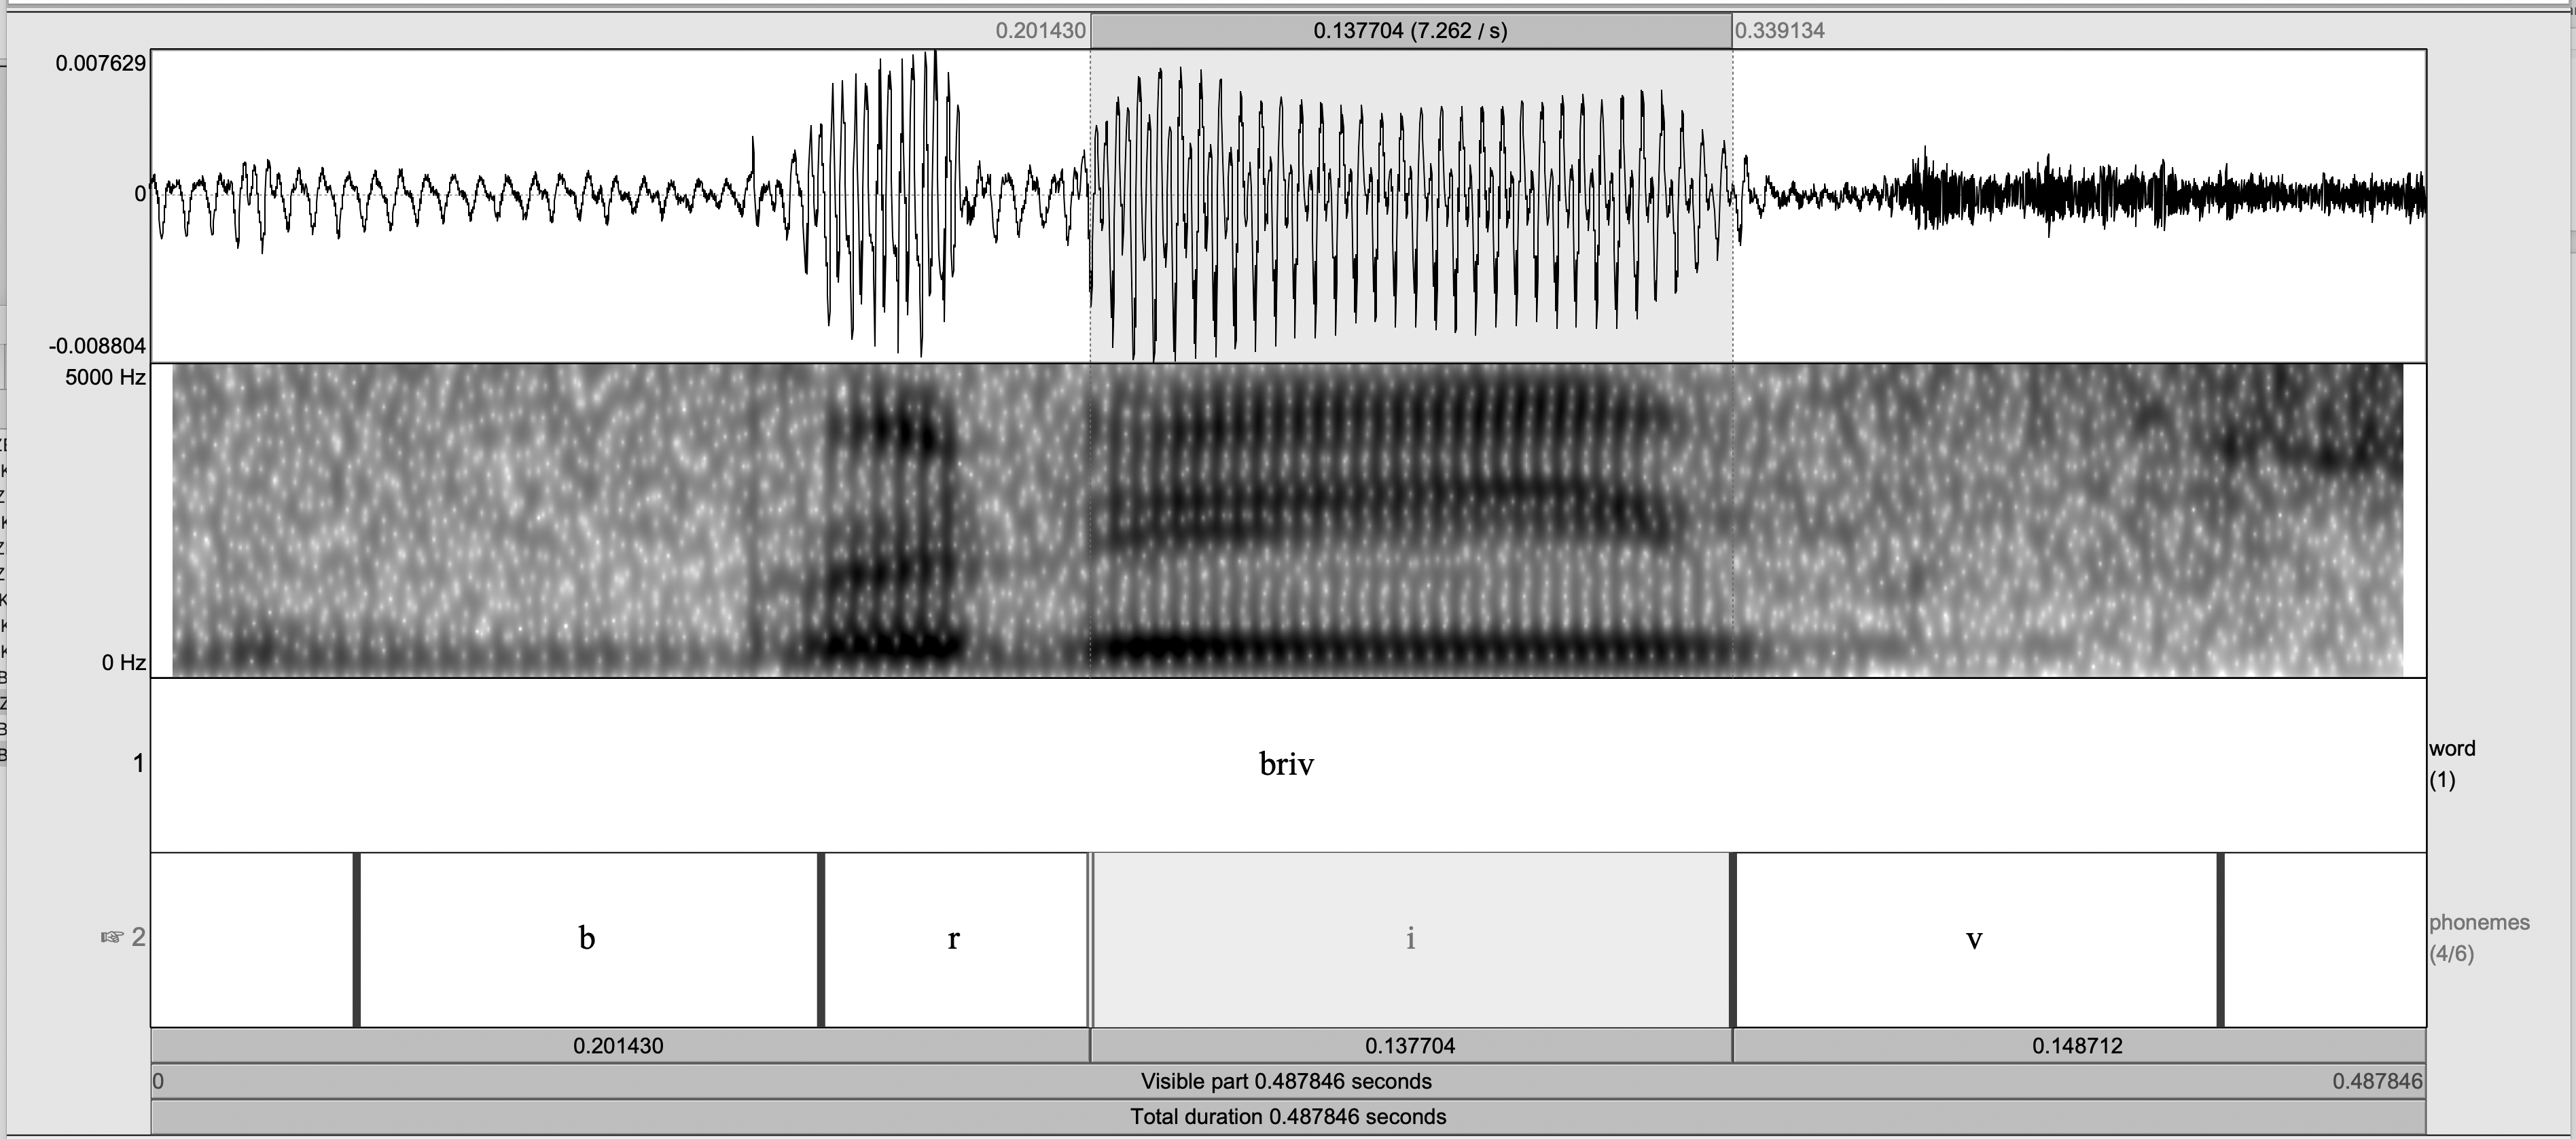
\includegraphics[width=\textwidth]{figures/nove-fig4-bw.png}
\caption{Waveform and spectrogram for the word <briv> ‘letter,’ by time (on the horizontal axis) and frequency (in Hz, on the vertical axis), with annotation showing the start and end points of individual segments. The speaker is 3B (39 years old, Gen3)}
\label{fig:nove:4}
\end{figure} 

 
  
%%please move the includegraphics inside the {figure} environment
%%\includegraphics[width=\textwidth]{figures/a03Nove-img004.png}
 

 \begin{figure}
 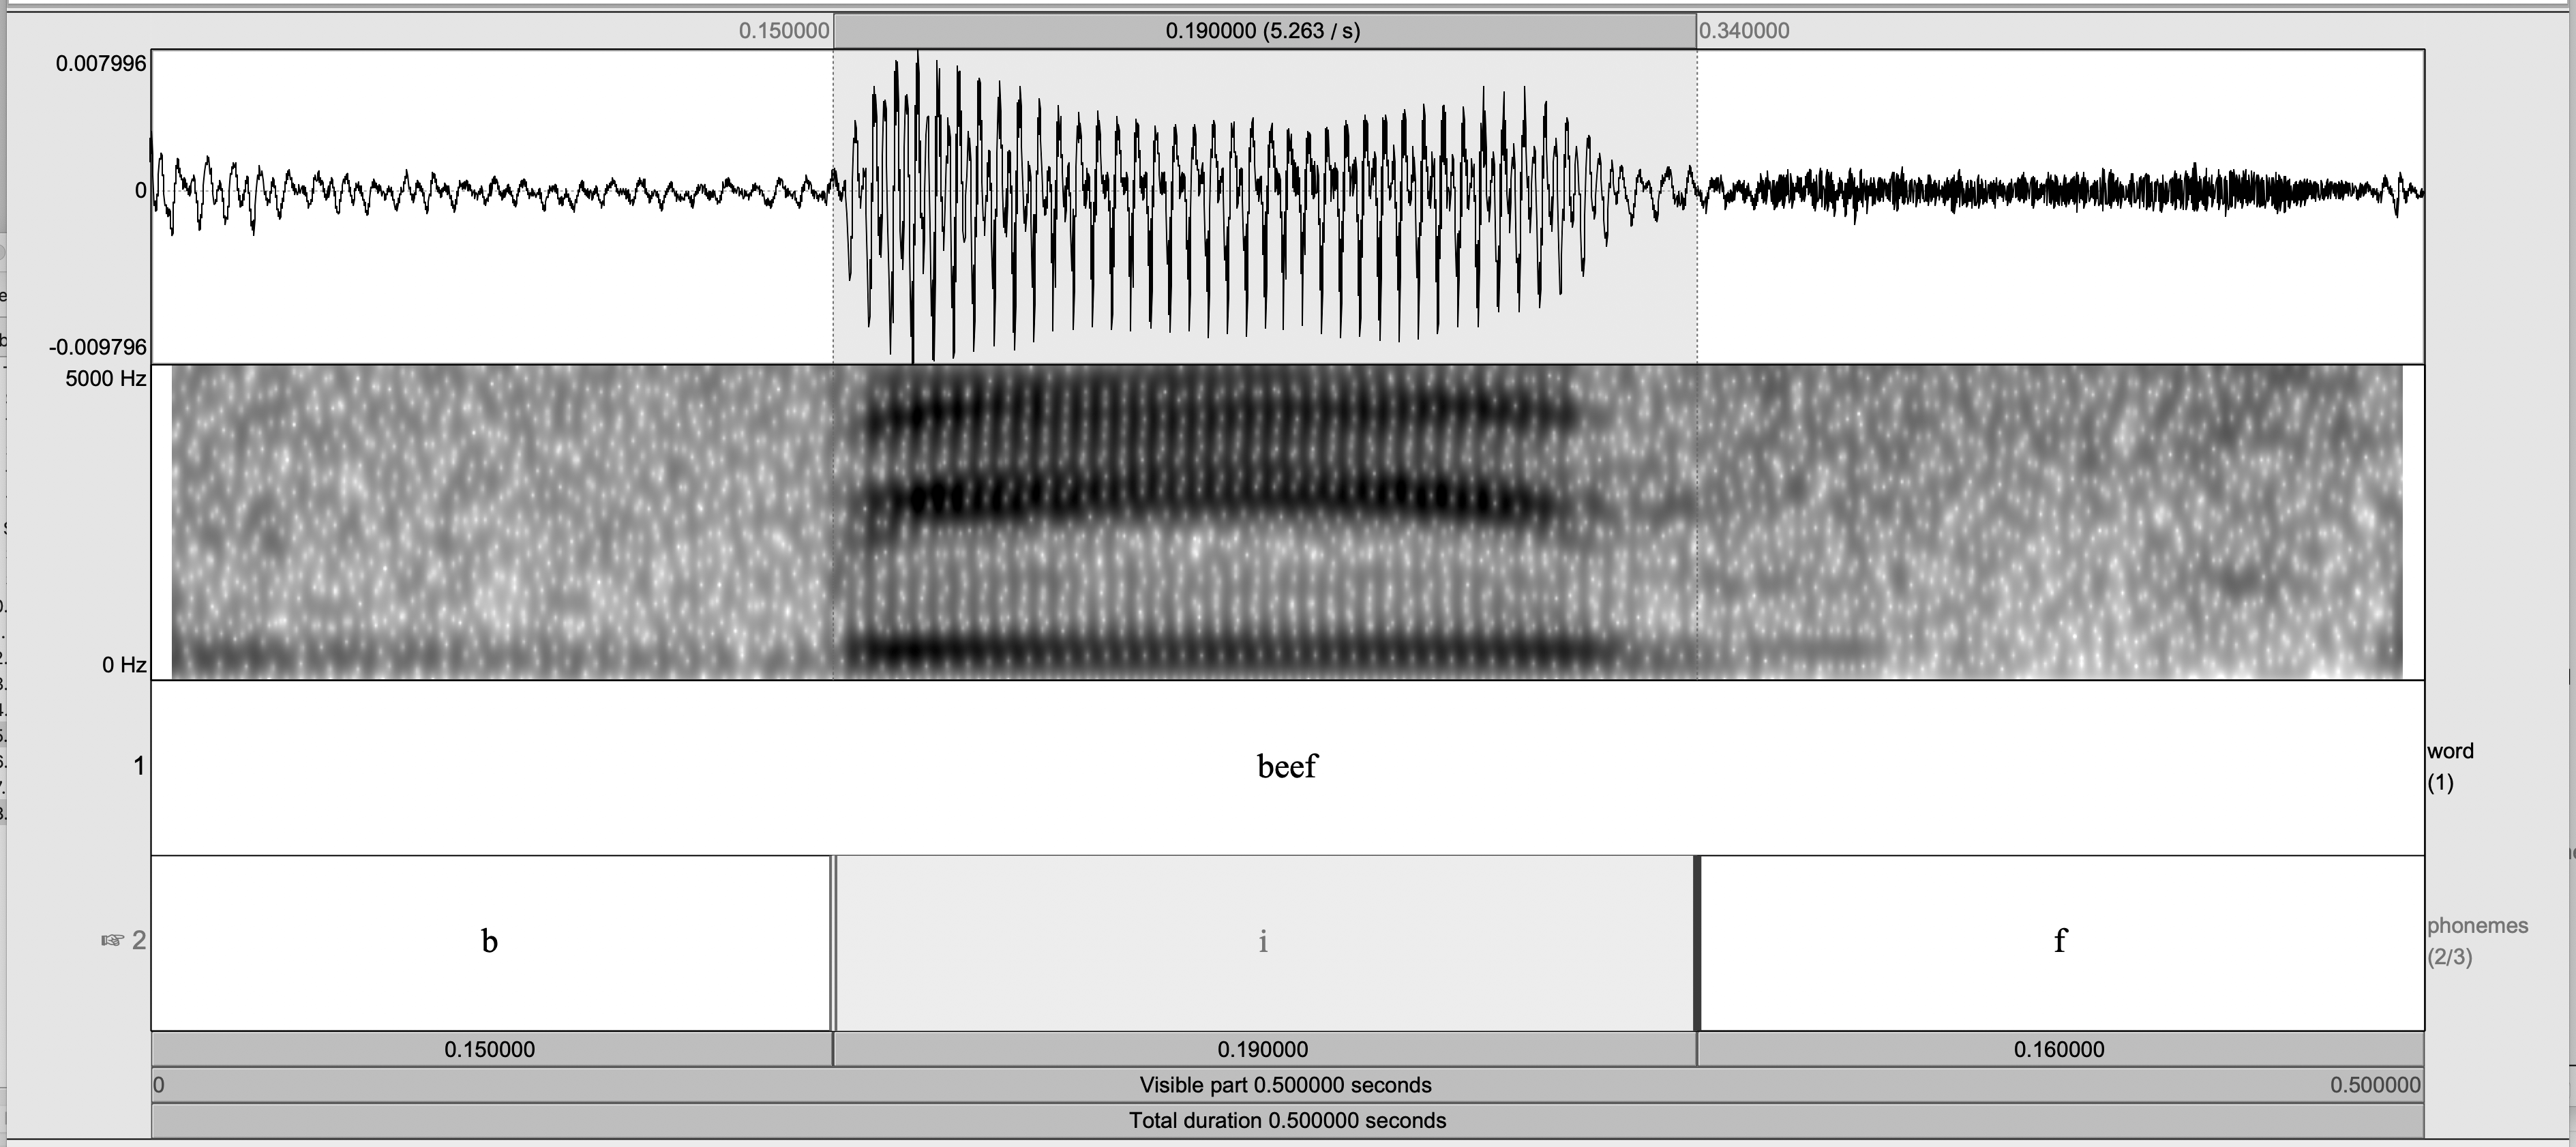
\includegraphics[width=\textwidth]{figures/nove-fig5-bw.png}
\caption{Waveform and spectrogram for the word <beef> by time (on the horizontal axis) and frequency (in Hz, on the vertical axis), with annotation showing the start and end points of individual segments. The speaker is 3B (39 years old, Gen3)}
\label{fig:nove:5}
\end{figure} 

Vowel tokens were extracted from the audio files and divided into three increments. The mean first and second formant (F1 and F2) frequencies of the second increment were measured from an LPC analysis over a 25-millisecond window with a 10-millisecond frame interval, using a script by \citet{Kang2016}. Formant measures were checked, and outlying values were manually corrected by visual inspection of a wideband spectrogram or discarded if formants could not be measured with certainty. Plots were created using the \textit{ggplot2} package \citep{Wickham2009} in R (\citealt{RCore2017}). The number of tokens extracted for each generational group are shown in \tabref{tab:nove:2} alongside mean F1 and F2 values of each word class by language.

\begin{table}
\begin{tabularx}{0.96\textwidth}{p{0.7cm}Xp{0.5cm}p{1.2cm}p{1.2cm}p{0.7cm}p{1.2cm}p{1.2cm}}
\lsptoprule
	& & ENG & & & HY & &\\
\cline{3-8}
{Vowel} & {Generation} & {n} & {F1} & {F2} & {n} & {F1} & {F2}\\
\hline
i & 2 & 78 & 334.48 & 2735.07 & 94 & 361.34 & 2649.76\\
i & 3 & 77 & 331.83 & 2492.11 & 91 & 340.26 & 2498.13\\
i & 4 & 88 & 393.16 & 2683.09 & 131 & 390.82 & 2654.51\\
ɪ & 2 & 87 & 473.61 & 2176.46 & 107 & 450.14 & 2289.92\\
ɪ & 3 & 87 & 471.10 & 2043.82 & 104 & 448.85 & 2082.91\\
ɪ & 4 & 109 & 491.60 & 2268.14 & 122 & 477.70 & 2171.98\\
u & 2 & 78 & 370.58 & 871.70 & 82 & 410.02 & 917.31\\
u & 3 & 77 & 370.40 & 1032.85 & 90 & 377.30 & 976.46\\
u & 4 & 96 & 406.60 & 1171.06 & 100 & 409.20 & 1054.01\\
ʊ & 2 & 79 & 501.26 & 1232.95 & 71 & 461.57 & 1108.55\\
ʊ & 3 & 80 & 493.54 & 1208.19 & 74 & 460.55 & 1147.63\\
ʊ & 4 & 94 & 538.32 & 1349.03 & 79 & 514.33 & 1333.98\\
a & 2 & 81 & 783.05 & 1408.58 & 87 & 822.50 & 1377.38\\
a & 3 & 87 & 762.31 & 1312.04 & 87 & 759.24 & 1319.03\\
a & 4 & 111 & 759.33 & 1506.28 & 103 & 778.33 & 1480.10\\
\lspbottomrule
\end{tabularx}
\caption{Mean formant frequencies of all vowel tokens by word class, generation, and language}\label{tab:nove:2}
\end{table}

Formant values (Hz) were normalized using the modified Watt \& Fabricius method as implemented in the \textit{phonR} package \citep{McCloy2016} in \textit{R}. This normalization method has been shown to reduce disparities caused by physiological factors and improve vowel space overlap for multiple speakers, while preserving socially and dialectally-induced differences in vowel quality (\citealt{WattFabricius2002, FabriciusEtAl2009}). Raw formant values and normalized values were then plotted and compared to check for distortion or artifacts introduced by normalization. 

Next, conventional vowel plots (F2 on the x-axis and F1 on the y-axis) were created to enable visualization of the data by language, separately for each generation. These are presented in \figref{fig:nove:6}. \figref{fig:nove:7} displays similar vowel plots created for each generational group by gender. The tokens were then plotted by vowel for each generation using two-dimensional contour maps, as shown in \figref{fig:nove:8}, in which density, represented by lines, is given as an additional dimension of the distribution of the vowel tokens.\footnote{Density maps rely on kernel density estimation (KDE), a non-parametric method of estimating the probability density function of a random variable. Given that a prior distribution is not assumed, they have the advantage of non-symmetry (see \citealt{NyczHall-Lew2013})} Finally, Pillai scores were calculated by generation for each vowel category, and by gender within each generational cohort, to measure the extent of overlap across and within languages. The Pillai score (or the Pillai-Bartlett trace), first applied to vowel overlap by \citet{HayEtAl2006} and elaborated on by \citet{NyczHall-Lew2013}, is the output of a MANOVA model/test,\footnote{A MANOVA is a type of analysis of variance that models two or more continuous dependent variables simultaneously to test whether they come from the same distribution in that multivariate space.} with F1 and F2 values entered as dependent variables. Pillai scores measure overlap by comparing the size and shape of word class clusters. The value of the scores ranges from 0 to 1, with 0 indicating total overlap between two clusters and 1 indicating no overlap. Manner and place of articulation of the preceding and following segments, as well as the duration of the vowel token, were included in the models as independent variables.

Sociolinguists studying the phonetic quality of North American English vowels have identified an implicational hierarchy in the vowel /u/ by context, which has led to a partition into three main lexical sets: 1) TOO: /u/ following coronal consonants tend to be the most advanced (fronted); 2) COOL: /u/ preceding laterals are the least advanced (backed); and 3) HOOP: /u/ elsewhere (\citealt{Hall-Lew2009, LabovEtAl2005, Baranowski2008}). To account for these systematic contextual differences, crosslinguistic Pillai scores for /u/ were calculated separately by lexical set. These are shown in \tabref{tab:nove:3} and \tabref{tab:nove:4}. As the Yiddish wordlist did not include tokens of COOL, only TOO and HOOP are compared. Additionally, within-language Pillai scores were obtained to compare TOO vs. HOOP in each generational group, as shown in \tabref{tab:nove:5}. 


 
 \subsection{Results}
\label{sec:nove:4.3}

In examining \figref{fig:nove:6}, below, we observe that the vowel plots of Gen2 appear to represent two distinct systems. In the HY system, the long-short versions of the high vowels ellipses overlap considerably, and the formant means are closer together, while the same vowels in the English system show minimal elliptical overlap and more distance between the formant means. The plot of Gen3 and Gen4 vowels illustrate a higher degree of similarity between the two languages, although the vowels of Gen4 show greater variability overall. The cross-generational difference in overlap of the high vowel pairs appear to be caused primarily by dissimilarities in the quality of the HY short/lax vowel in each pair. That is, Gen2 HY /ɪ/ and /ʊ/ are higher (larger F1 values) and more peripheral (F2 values are lower for /ɪ/ and higher /ʊ/) than Gen2 and Gen3, but the corresponding English vowels occupy similar positions for all generations. There are no discernible differences in the phonetic positions of /i/ and /a/ across languages or generations. 


\begin{figure}
 %%please move the includegraphics inside the {figure} environment
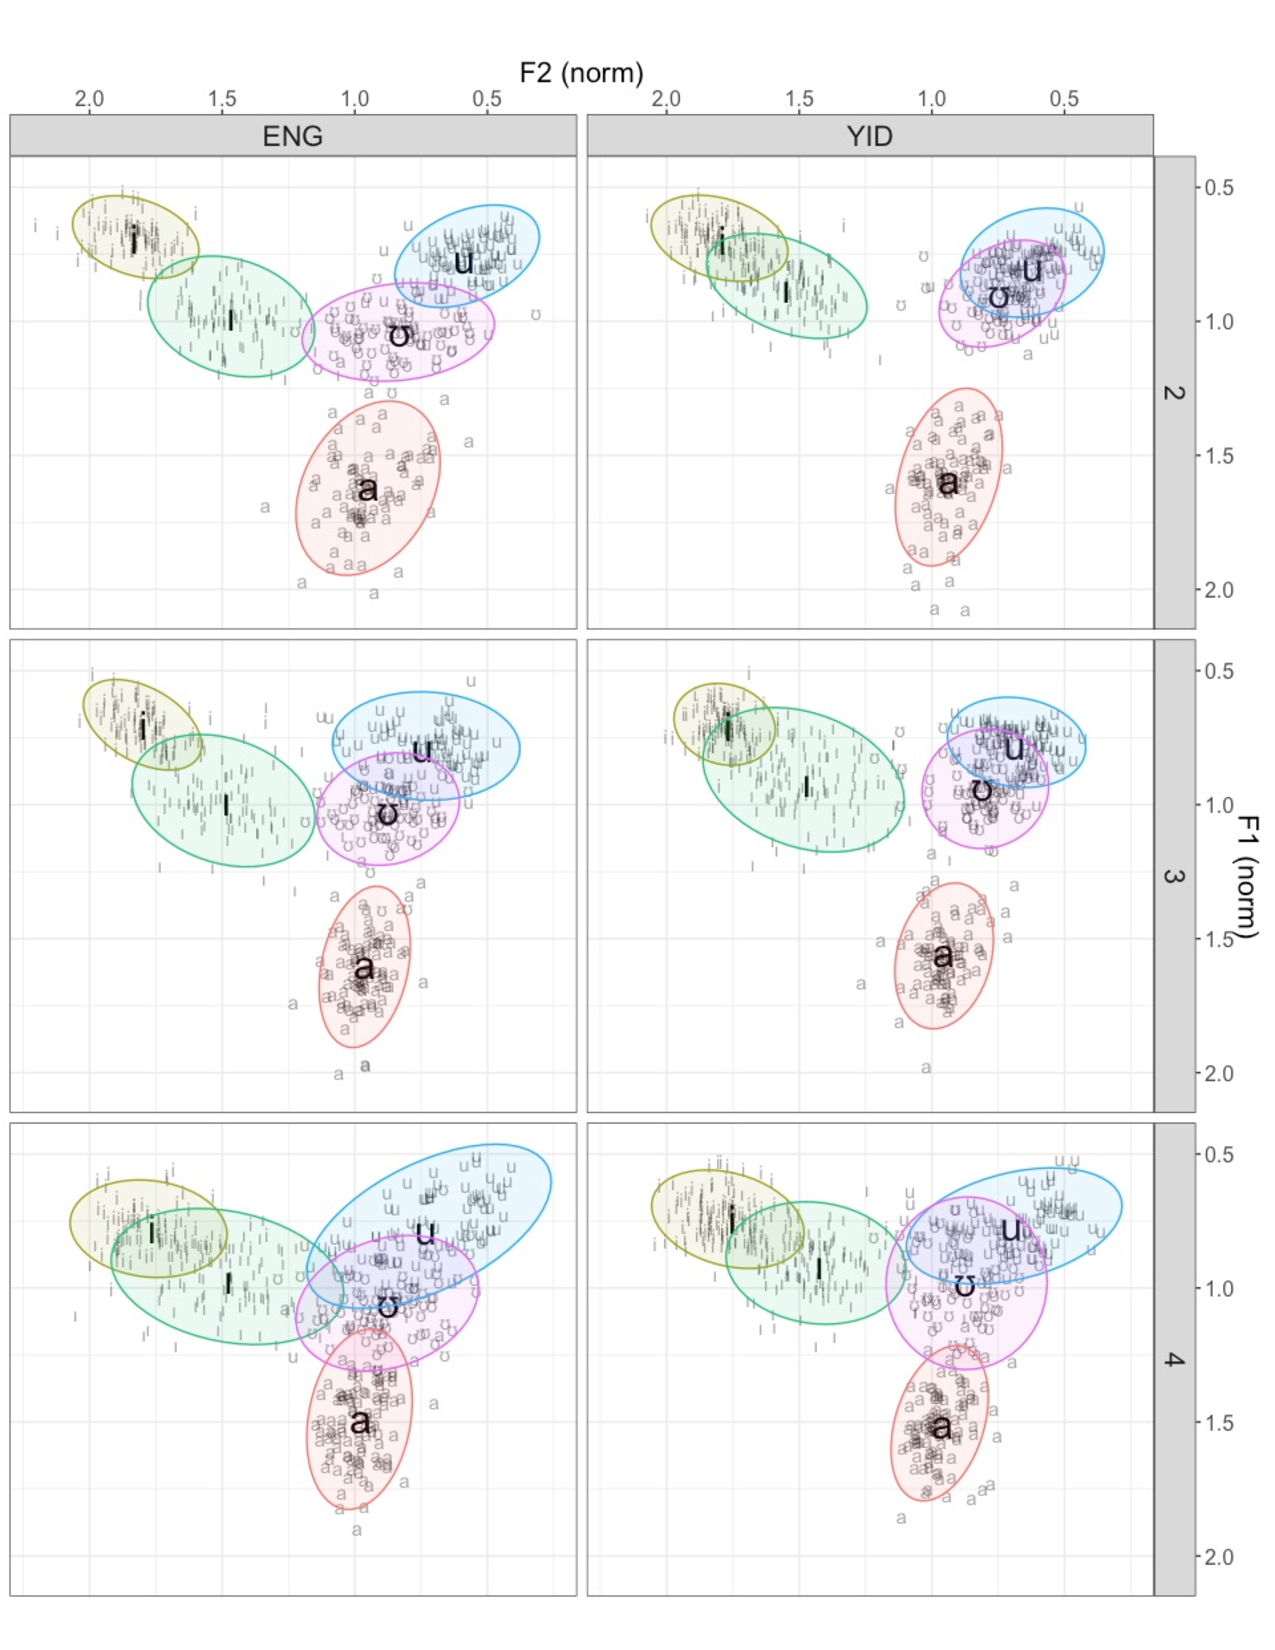
\includegraphics[width=\textwidth]{figures/nove-fig6_color.pdf}
\caption{Plots of normalized F1 and F2 values of all vowel tokens, faceted by generation (rows) and language (columns), with HY labeled “YID.” Formant means are represented by symbols in large font. Ellipses represent 95\% confidence intervals. N = 2577 (HY = 1367; ENG = 1210)}\label{fig:nove:6}
\end{figure} 

When the data of each generational cohort are plotted separately by gender (\figref{fig:nove:7}), a slight discrepancy is visible between female and male speakers of the Gen2, with female speakers showing more variability and greater cross-linguistic overlap in the short high vowels. This gender difference shows up in the Pillai scores calculated by gender (see \tabref{tab:nove:3}, below): For both short high vowels (ɪ and ʊ), male speakers have higher values than female speakers, indicating more separation between the HY and English clusters. In the younger generational groups, there is a small difference in the scores of /ʊ/ in Gen4 females and males in the opposite direction, suggesting greater cross-linguistic overlap among male speakers. 


\begin{figure}
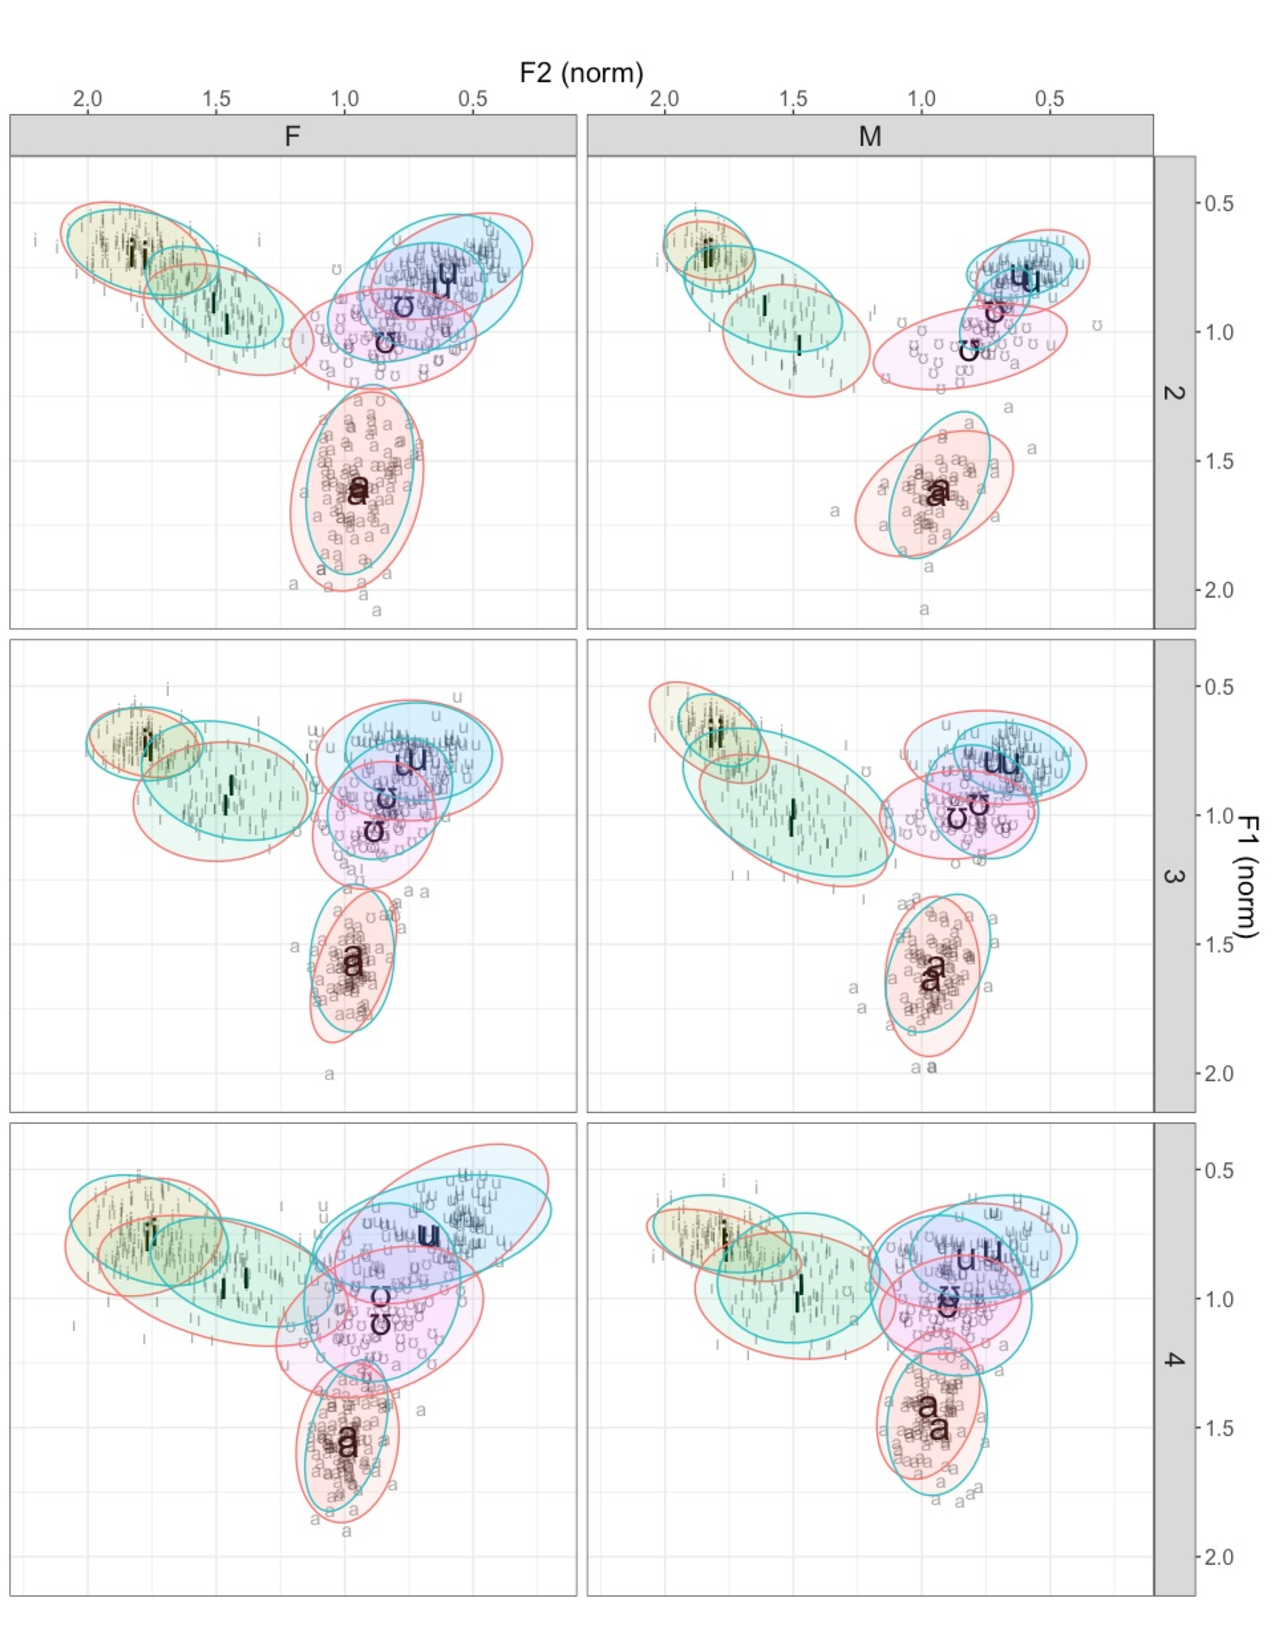
\includegraphics[width=\textwidth]{figures/nove-fig7-color.pdf}
\caption{Plots of normalized F1 and F2 values of all vowel tokens, grouped by language and faceted by generation (rows) and gender (columns). Dashed outlines indicate HY vowels and smooth outlines English vowels.}\label{fig:nove:7}
\end{figure}

\begin{table}
\begin{tabularx}{\textwidth}{XXXXXXXX}
\lsptoprule
Gen & Sex & /i/ & /ɪ/ & HOOP  & TOO  & /ʊ/  & /a/ \\
\hline
2 & F & 0.05 & 0.24 *** & 0.28 ** & 0.04 & 0.38 *** & 0.02 \\
2 & M & 0.03 & 0.60 *** & 0.06 & 0.06 & 0.66 *** & 0.01  \\
3 & F & 0.02 & 0.16 *** & 0.31 ** & 0.34 *** & 0.29 *** & 0.03 \\
3 & M & 0.09 & 0.12 ** & 0.15 & 0.41 *** & 0.24 ** & 0.09  \\
4 & F & 0.03 & 0.18 *** & 0.02 * & 0.05 & 0.23 ** & 0.09 *\\
4 & M & 0.17 & 0.10 * & 0.38 ** & 0.28 ** & 0.06 & 0.17 **\\
\lspbottomrule
\end{tabularx}
\caption{Crosslinguistic Pillai scores by vowel/set, grouped by generation (Gen) and sex. Significance codes: *** = <0.001, ** = <0.01, * = <0.05, . = <0.1}
\label{tab:nove:3}
\end{table}

Next, we consider the extent of crosslinguistic overlap as represented by the contour maps for each vowel (\figref{fig:nove:8}). The plots representing tokens of /i/ and /a/ show the distribution of the HY and English vowels essentially overlapping for all generations, that is, there is minimal phonetic difference between them. This observation is confirmed by the Pillai scores for these vowels (shown in \tabref{tab:nove:4}), which are smaller than 0.1, for all generations, with differences of only 0.02--0.04 points between groups. With the exception of Gen4 /a/, these differences are also not statistically significant. The representation is different for the short-lax vowels /ɪ/ and /ʊ/. Here we see quite a bit of separation in the HY vs. English vowels of Gen2 on both axes (F1 and F2). Spectrally, they are more distinct in the oldest generation, with the HY cluster situated closer to the periphery. The following generations show increasing overlap in these vowels, especially /ɪ/. We see a reflection of this in the Pillai scores, with the Gen2 exhibiting scores for /ɪ/ and /ʊ/ that are significantly higher (.33 and .45, respectively) than for the other two groups.


\begin{figure}
%please move the includegraphics inside the {figure} environment
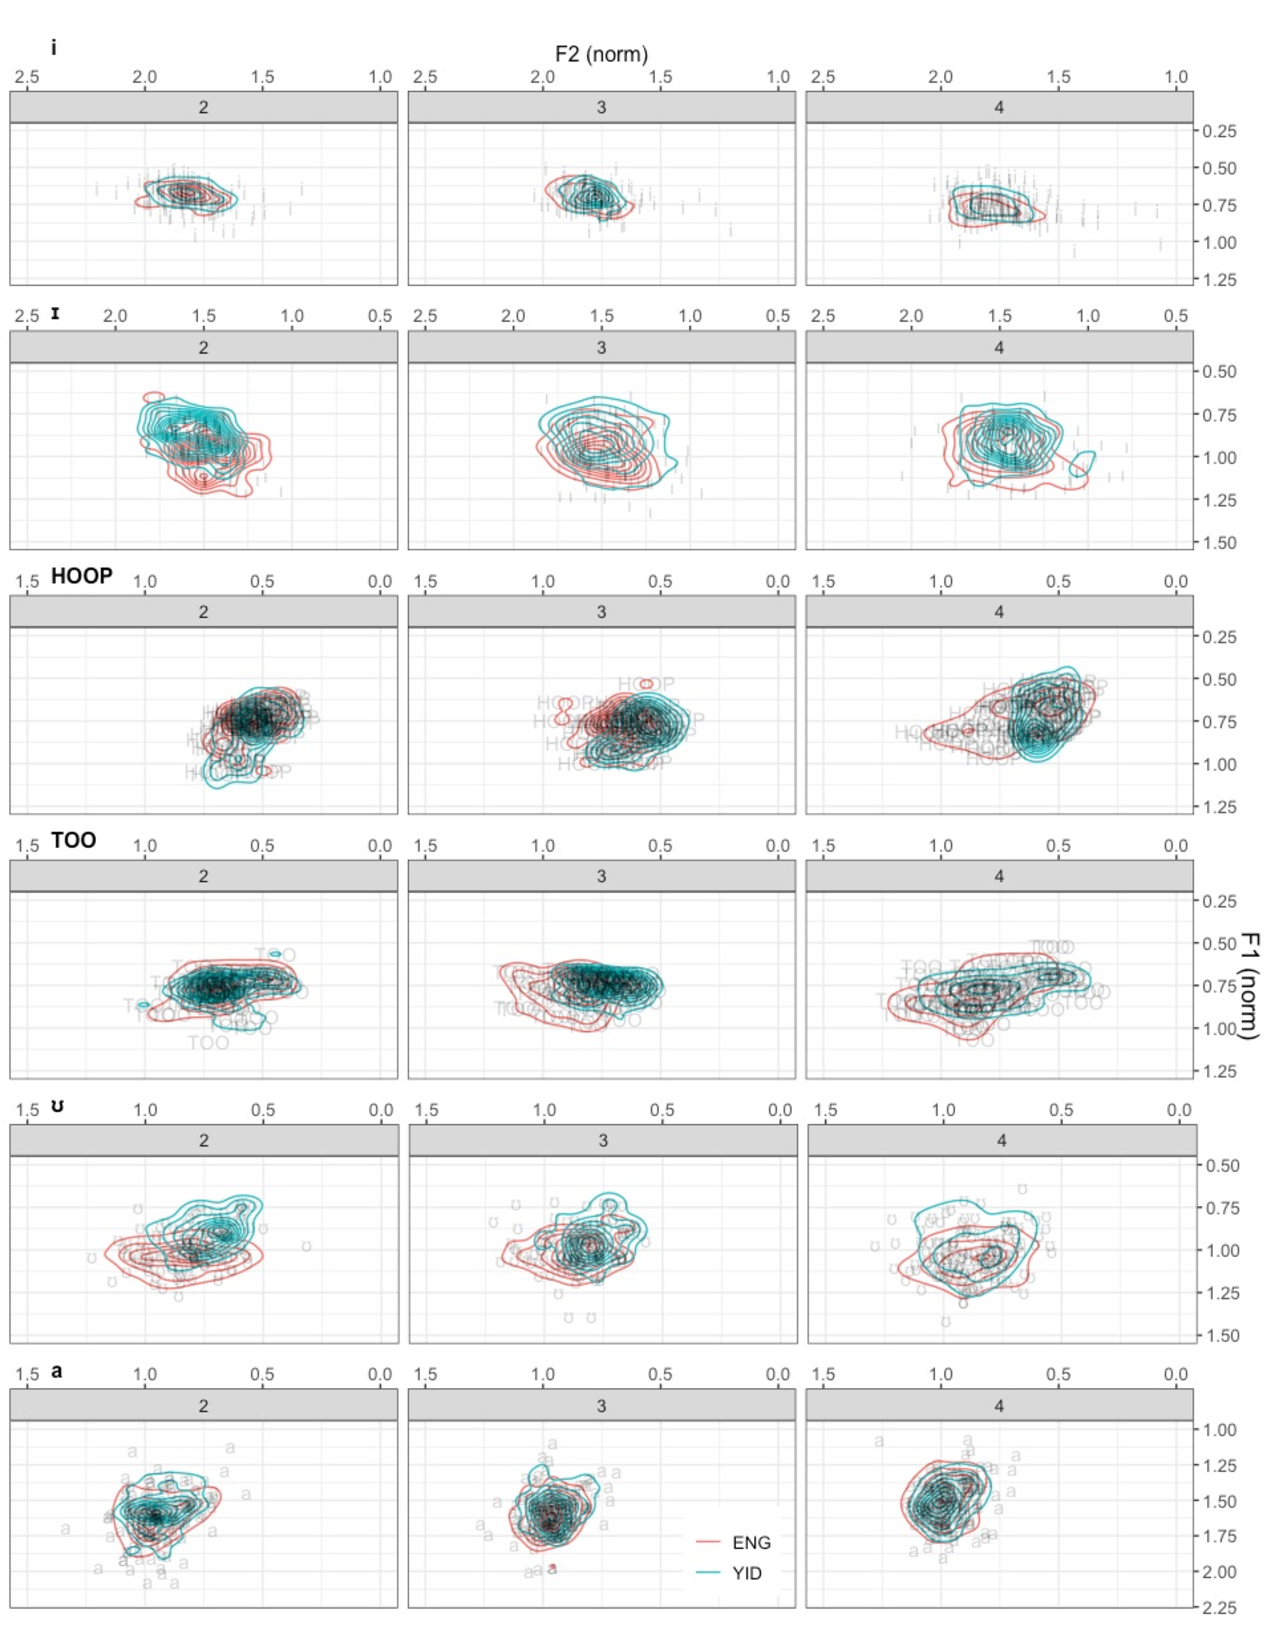
\includegraphics[width=\textwidth]{figures/nove-fig8-color.pdf}
\caption{Contour plots of all vowels showing location (by normalized F1 and F2) and density, faceted by generational group}
\label{fig:nove:8}
\end{figure}

\begin{table}
\begin{tabularx}{\textwidth}{XXXXXXX} 
\lsptoprule
& /i/ & /ɪ/ &  HOOP &  TOO &  /ʊ/ &  /a/ \\
\hline
Gen2 & 0.04 . & 0.33 *** & 0.09 . & 0.00  & 0.45 *** & 0.01 .\\
Gen3 & 0.02 & 0.07 ** & 0.16 ** & 0.39 *** & 0.23 *** & 0.03  \\
Gen4 & 0.06  & 0.11 *** & 0.12 * & 0.08 * & 0.12 *** & 0.03  \\
\lspbottomrule
\end{tabularx}
\caption{Crosslinguistic Pillai scores by vowel/set for each generational. Significance codes: *** = <0.001, ** = <0.01, * = <0.05, . = <0.1}\label{tab:nove:4}
\end{table}

Finally, we turn to the long high back vowels, which were calculated separately for the lexical sets TOO and HOOP. Here, the first finding is that Gen2 exhibits more F2 overlap than the younger generations, whose HY-English vowel tokens are slightly separated along the F2 (\figref{fig:nove:8}). That is, English TOO and HOOP of Gen3 and Gen4 are a bit more advanced than the HY counterparts. Pillai scores once again reflect this distribution, although the differences are small. Within-language statistical comparisons of these vowels by set (\tabref{tab:nove:5}) shows that TOO is slightly more advanced than HOOP in both languages for all speaker groups.

\begin{table}
\begin{tabularx}{0.6\textwidth}{XXX}
\lsptoprule 
 & {HY} & {ENG} \\
\hline
Gen2 & 0.27 *** & 0.336 ***\\
Gen3 & 0.39 {***} & 0.536 {***}\\
Gen4 & 0.23 {***} & 0.338 {***}\\
\lspbottomrule
\end{tabularx}
\caption{Within language Pillai scores by lexical set (HOOP vs. TOO) for each generational group. Significance codes: *** = <0.001, ** = <0.01, * = <0.05, . = <0.1}
\label{tab:nove:5}
\end{table}

The differences in advancement of TOO vs. HOOP in HY are in line with the patterns found between these lexical sets in North American English (i.e., TOO is more advanced than HOOP), however, it is notable that the mean F2 values of both HY and English TOO are considerably lower (less than 1200 Hz) in this speaker group than the values typically found among mainstream New York English speakers (around 1800 Hz for New York City, see \citealt{Newman2014}; \citealt{Wong2014}; \citealt{HaddicanEtAl2019}). Moreover, more fronting is visible in the HY TOO of Gen4 than of the older generations.

Finally, while the Pillai scores calculated by gender also suggest greater separation of HY vs. English HOOP for male speakers of Gen2 and Gen3, and the reverse for Gen4, no clear patterns emerged when these data were visualized via a variety of plots and graphs, most likely due to the relatively small sample size (female vs. male speakers by group) and limited number of tokens in each category. Further research, which includes a larger sample size and both conversational and wordlist data, is in progress. 


\section{Discussion} 
\label{sec:nove:5}

The results obtained in this comparative study provide evidence of apparent time change between Gen2 and Gen3/Gen4 in the spectral overlap of HY-English /ɪ/ and /ʊ/ and the relative advancement of English vs. HY /u/. As described in \sectref{sec:nove:4.3}, Gen2 speakers exhibit different organizations of their HY and English high vowels: While the HY short high vowels /ɪ/ and /ʊ/ are qualitatively more similar to their tense counterparts /i/ and /u/ (i.e., the vowels in each pair are closer in phonetic space), the equivalent English vowel pairs are more distinct. Moreover, the separation is more pronounced among Gen2 male than female speakers. These cross-linguistic differences in the vowel system of Gen2 gradually diminish in the younger generational cohorts. The reverse pattern holds for the qualitative similarity of /u/ (TOO and HOOP) across languages. Here, the younger generations exhibit less overlap than Gen2, with more fronted English /u/ tokens.

In hypothesizing about the source of these cross-generational differences, we consider \citegen{Flege2007} contention about the significance of input in L2 learning outcomes. Recall that Gen2 speakers are children of post-Holocaust immigrants to the U.S. All those interviewed for this study were, in fact, born within five years of their parents’ arrival, a period during which these immigrant parents would probably not yet have acquired English. Thus, the Yiddish input for Gen2 was Unterland Yiddish, in which the contrast in the peripheral vowels is primarily duration, rather than quality (see \citealt{Nove2020}). Their English input, however, came largely from non-Yiddish speakers.\footnote{Field notes and sociolinguistic interviews, 2017--2019.} Given the differences in the phonetic contrast of the vowel pairs \{/i/, /ɪ/\} and \{/u/, /ʊ/\} in Unterland Yiddish vs. mainstream American English, namely, a length contrast in the former and a qualitative (tense-lax) distinction in the latter, Gen2 speakers likely perceived and classified them as different vowels, thus leading to the different systems observed in \figref{fig:nove:6}. However, keeping in mind that these speakers were in their 60s and 70s when they were recorded for this study, change across the lifespan should not be ruled out. That is, it is reasonable to hypothesize that the short vowels of Gen2 may have resembled those of their parents more closely at a younger age, and that phonetic drift (a shift in the phonetic quality of a sound segment, influenced by speakers’ experience with English) resulted in a slight lowering and centralizing of HY /ɪ/ and /ʊ/ at the individual level over time. Such an outcome is predicted by the SLM and is well documented in the literature (see review by \citealt{Chang2019}). Moreover, male Gen2 speakers, who acquired English later and used it less frequently than their female contemporaries, likely started out with more conservative HY vowels (i.e., tenser high short vowels) and maintained the cross-linguistic separation of the vowel systems more fully.\footnote{Although gender differences are not immediately apparent for Gen3 and Gen4 speakers in the analyses provided here, their existence should not be ruled out. While Pillai scores measure overlap, they do not show directionality of vowel movement. Thus, this analysis may not reveal effects such as differential L1 – L2 influence. That is, it may turn out that while the amount of cross-linguistic overlap in the male vs. female speakers is relatively consistent, in one group (or in some individuals) this overlap is due to HY vowel lowering and in the other to ENG vowel raising. Future analyses that include a larger sample size and additional statistical models are in progress to investigate these in greater detail.} The comparatively laxer (more centralized) HY vowels of Gen2, in turn, served as the HY input for Gen3 and Gen4, who acquired their English from other HY-English bilinguals in their community. In accordance with the SLM, the ‘similar’ HY and English /ɪ/ and /ʊ/ sound segments were likely perceived as equivalent by speakers of the younger generations, and thus acquired with the same phonetic values, leading to the crosslinguistic phonological convergence that we observe in the data. %The potential influence of language input is also highlighted by Stuhl (this volume) for Namdeutsch, who cites the growing presence of Standard German, via media, education, and travel, as a reason why the phonology may be shifting towards the standard.
The potential influence of language input is also highlighted by \citetv{chapters/04_stuhl} for Namdeutsch, who cites the growing presence of Standard German, via media, education, and travel, as a reason why the phonology may be shifting towards the standard.

Factor The comparatively low F2 values of both HY and English /u/ in this community, on average lower than 1200 Hz, indicates either a lack of participation, or a significant lag, in the u-fronting trend that has been observed in the majority population. This can be interpreted as an L1 influence, i.e., the relative backness of HY vowels exerting a retractive influence on the English vowels of these bilingual speakers. Alternatively, speakers in this community might be somewhat insulated from the sound changes occurring among mainstream English speakers by virtue of their sociocultural separateness \citep{Fader2009}. A similar phenomenon, described by \citep{Benor2009, Benor2012}, is the comparatively lower/laxer quality of prenasal /æ/ among Orthodox Jews, indicating a lack of participation in prenasal /æ/-tensing, a prevalent sound change among mainstream American English speakers. The relative advancement of Gen3 and Gen4 English /u/ suggests that u-fronting may indeed be permeating this speech community but is still at an early stage. Moreover, the finding that Gen4 HY TOO is slightly more fronted than the older generations, possibly signifies another instance of phonetic drift, i.e., HY u-fronting under the influence of English. 

As described in \sectref{sec:nove:1}, New York HY severed all ties with its homeland dialect more than seven decades ago, when it was transplanted to the U.S. along with its refugee speakers. Sustained by an ideology that supports language maintenance, it is still far from immune to the cognitive, linguistic and social influences of the majority language. But how does such vulnerability translate into language change? The analysis and interpretation provided here illustrate how an understanding of the dynamic nature of the language systems of individual learners can help explain structural change observed in the language of a speech community. 

\section*{Appendix}\label{sec:nove:appendix}


\begin{table}
\fittable{
\footnotesize
\begin{tabularx}{\textwidth}{p{1.5cm}XXXXXXXXXX}
\lsptoprule 
 \textsc{poa} & \textsc{eng} & \textsc{hy} & \textsc{eng} & \textsc{hy} & \textsc{eng} & \textsc{hy} & \textsc{eng} & \textsc{hy} & \textsc{eng} & \textsc{hy} \\
 \cmidrule{2-11}
 & \multicolumn{2}{c}{/i/} & \multicolumn{2}{c}{/ɪ/} & \multicolumn{2}{c}{/u/} & \multicolumn{2}{c}{/ʊ/} & \multicolumn{2}{c}{/a/} \\
\hline
 Non-lingual
(bilabial, labio-dental) & beef seep sleeve & tiif shiif liib briiv & 	shift gift tip & shif lip & snoop & shtruuf & & grub tuf shluf & mop top mob & khap\\
\hline
Coronal & meet sheet geese weed feel teal
& hiit giis miis miid ziin tiir fiil & hit miss hid sing dim fill
 & hit git miz tish zin din zing fil & hoot suit food rude mood noose moose boon pool & bruut ruut shtuut muus gruud gruuz fuun nuunt kluur tsuul & foot put hood should good would pull & vus & pot lot hot dots rod nod & zat bas dan hant man vant fal kalt sharf\\
 \hline
Dorsal & geek & ziikh kriig & pick big & dik kik lig
& & & took brook nook & tsuk frukht nukh yug nug zug & lock & pak
lakht\\	
\lspbottomrule
\end{tabularx}
\caption{Word lists for each vowel category by language, arranged by place of articulation of the consonant following the vowel. HY words are transliterated phonetically, with /u/ represented as <uu> and /i/ as <ii>}
\label{tab:nove:6}
}
\end{table}

As the wordlist task was initially designed to investigate the contrast in HY vowel pairs, the first consideration was to include as many minimal pairs within the HY (and later English) vowel sets (e.g., {[}zin{]}, {[}zɪn{]} for {/i/, /ɪ/}). Secondly, there was an attempt to match the contexts (especially the following consonant) of the English words with the Yiddish ones (e.g., the lexical item {[}hɪt{]}, which exists in both languages). Finally, attention was paid to include as many consonant classes as possible following the vowel, i.e., voicing (+/-), manner (voiceless obstruents, voiced obstruents, nasals, laterals and rhotics) and place (non-lingual, coronal and dorsal). Note that the split between long-short /u/ in Yiddish was historically conditioned by following segment: /u/ followed by velar or labial consonants became shortened. Thus, {[}u{]} is found before coronals and {[}ʊ{]} before dorsal and non-lingual segments. 
Some redundancy was built into the list and several adjustments were made after the study commenced, with some words removed and others added based on issues encountered, including word recognition difficulties and variable pronunciation.


{\sloppy\printbibliography[heading=subbibliography,notkeyword=this]}

\end{document} 
